\documentclass{beamer}
\mode<presentation>
\usetheme{CambridgeUS}
\usepackage[russian]{babel}
\usepackage[utf8]{inputenc}
\usepackage[T2A]{fontenc}
\usepackage{sansmathaccent}

\usepackage{verbatim}
\usepackage{alltt}

\pdfmapfile{+sansmathaccent.map}
\title[Шаблоны]{Шаблоны информационной архитектуры}
\author{Наумов Д.А., доц. каф. КТ}
\date[18.11.2020] {Компьютерная графика и проектирование графических интерфейсов, 2020}

\begin{document}

%ТИТУЛЬНЫЙ СЛАЙД
\begin{frame}
  \titlepage
\end{frame}
  
%СОДЕРЖАНИЕ ЛЕКЦИИ
\begin{frame}
  \frametitle{Содержание лекции}
  \tableofcontents  
\end{frame}

\section{Информационная архитектура, организация контента}

\begin{frame}[t]
	\textit{Высокоуровневая оганизация информации:}
	\begin{itemize}
		\item разделение сущностей -- отделение содержимого от физического представления;
		\item физическая структура -- представление материала на страницах.
	\end{itemize}
	
	Большинство приложений и многие веб-сайты организуются соглласно одному из нескольких следующих принципов:
	\begin{itemize}
		\item \textit{списки объектов} -- папка входящих сообщений;
		\item \textbf{списки действий или задач} -- посмотреть, приобрести, продать, зарегистрироваться; 		
		\item \textit{списки тематических категорий} -- здоровье, наука, технология;		
		\item \textit{списки инструментов} -- календарь, адресная книга, блокнот.		
	\end{itemize}
	
	Любую страницу можно рассматривать с точки зрения того, что оно долнжа делать:
	\begin{itemize}
		\item отобразить едиственный объект (карта, книга, видео, игра);
		\item отобразить список объектов;
		\item \textbf{предоставить возможность что-то сделать};
		\item \textbf{выполнить определенную задачу}.				
	\end{itemize}
\end{frame} 

\section{Действия и команды}

\begin{frame}[t]{Действия и команды}
	\textit{Как пользователи могут решать свои задачи, взаимодействуя с сайтом или приложением?}
	\begin{itemize}
		\item начать простановить, отменить или завершить действие;
		\item ввести значение, задать настройки;
		\item выполнить действие с объектом;
		\item применить изменения;
		\item удалить объект;				 		
		\item добавить/создать объект.		
	\end{itemize}
	
	Каждый <<интересный>> гарфический элемент для чего-то нужен.
	\begin{itemize}
		\item значки, объекты или формы, отличающиеся от остального контента;
		\item выделяющийся текст;
		\item объект, реагирущий на указатель мыши;
		\item объект, реагирующий на нажатие, поворот экрана;
	\end{itemize}		
\end{frame}

\begin{frame}[t]{}
	\begin{figure}[h]
		\centering
		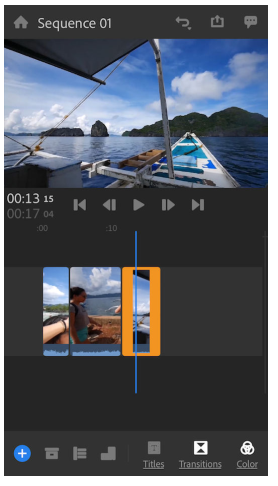
\includegraphics[scale=0.5]{images/lec08-pic01.png}
		\caption{Adobe Premier Rush}
	\end{figure}
\end{frame}	

\begin{frame}[t]{Windows Logo Evolution}
	\begin{figure}[h]
		\centering
		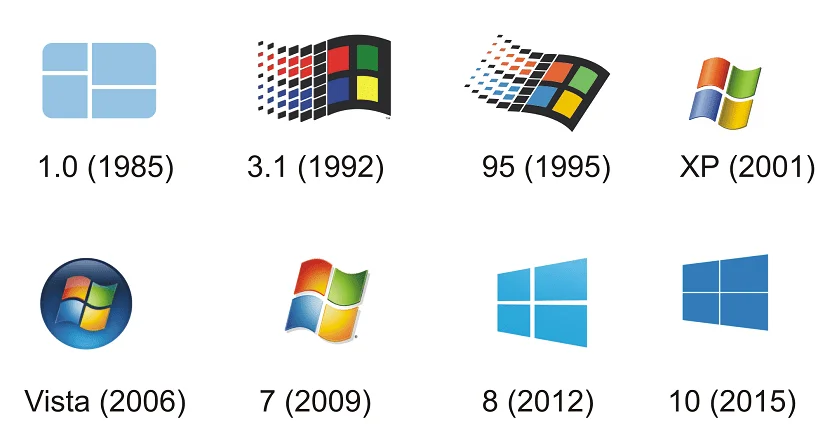
\includegraphics[scale=0.5]{images/windows_logo.png}
	\end{figure}
\end{frame}	

\begin{frame}[t]{Действия и команды}
	Тенденции в UI/UX:
	\begin{itemize}
		\item набор инструментов UI;
		\item библиотеки и фреймворки;
		\item набор компонент;
		\item отсутствие необходмости <<кодирования с нуля>>;
		\item стандартная функциональность:
		\begin{itemize}
			\item copy-paste
			\item drag-n-drop			
			\item tap, swipe, pinch			
			\item rotate and shake			
			\item buttons, pop-up, drop-down menu, toolbars
			\item links		
			\item single-click /double click				
			\item shortcuts			
			\item tab order			
		\end{itemize}
	\end{itemize}
\end{frame}

\section{Шаблоны для действий и команд}

\begin{frame}[t]{Button Groups}
	Есть много действий, они видны все время, но мам нужно их визуально организовать.

	\textbf{Шаблон}: группировать связанные действия в некий кластер.

	\begin{figure}[h]
		\centering
		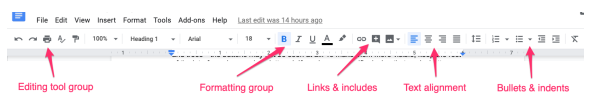
\includegraphics[scale=0.6]{images/lec08-pic02.png}
		\caption{Button Groups in Google Docs}
	\end{figure}
	\begin{figure}[h]
		\centering
		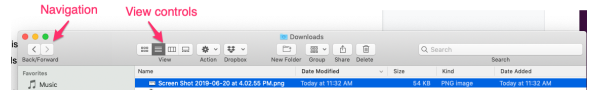
\includegraphics[scale=0.6]{images/lec08-pic03.png}
		\caption{Apple macOS Finder}
	\end{figure}	
\end{frame}	

\begin{frame}[t]{Hover or Pop-Up Tools}
	Есть много действий, но большую часть времени нужен чистый, незагроможденный контент. Мы хотем поместить действия куда-то, предпочтительно на объекты, с которыми они выполняют действие.

	\textbf{Шаблон}: Поместите кнопки и другие действия рядом с элементами, на которые они действуют, но спрячьте их, пока
пользователь не наведет на них указатель.
	\begin{figure}[h]
		\centering
		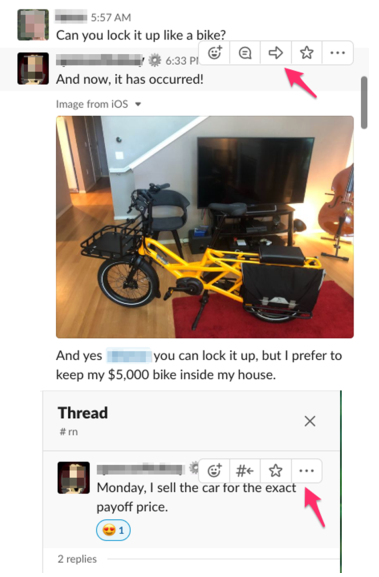
\includegraphics[scale=0.6]{images/lec08-pic04.png}
		\caption{Slack; examples of hover tools for posts and threads}
	\end{figure}
\end{frame}	

\begin{frame}[t]{Hover or Pop-Up Tools}
	\begin{figure}[h]
		\centering
		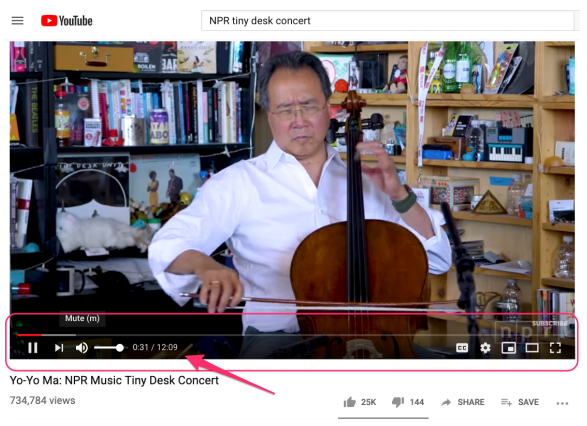
\includegraphics[scale=0.6]{images/lec08-pic05.png}
		\caption{YouTube web player}
	\end{figure}
\end{frame}

\begin{frame}[t]{Action Panel}
	Действий слишком много, чтобы показать все действия для каждого элемента, и слишком много для шаблона \textit{Hover}.

	\textbf{Шаблон}: Панель команд
		\begin{itemize}
		\item можно предлагать наиболее распространенные действия;
		\item можно отображать наиболее подходящие команды.
	\end{itemize}
	
	\begin{figure}[h]
		\centering
		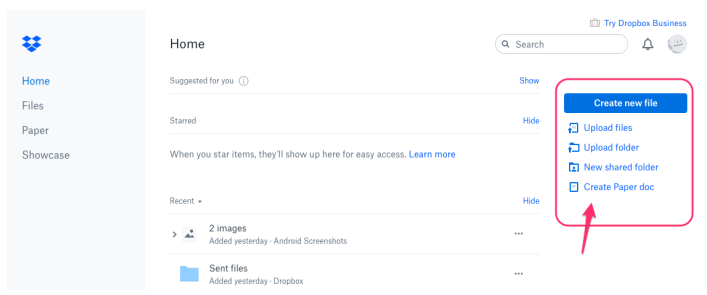
\includegraphics[scale=0.5]{images/lec08-pic06.png}
		\caption{An Action Panel in Dropbox}
	\end{figure}
\end{frame}

\begin{frame}[t]{Action Panel}
	\begin{figure}[h]
		\centering
		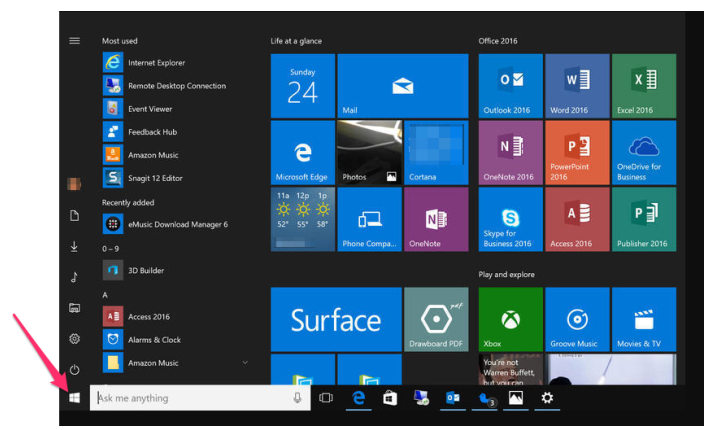
\includegraphics[scale=0.5]{images/lec08-pic07.png}
		\caption{Microsof Windows 10 Start Menu}
	\end{figure}
\end{frame}

\begin{frame}[t]{Action Panel}
	\begin{figure}[h]
		\centering
		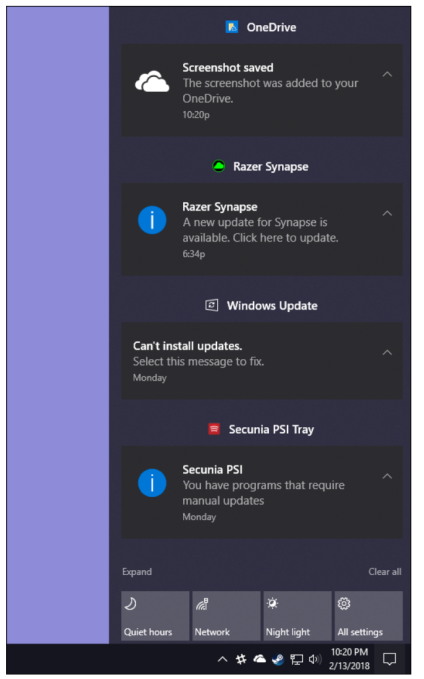
\includegraphics[scale=0.4]{images/lec08-pic08.png}
		\caption{Microsof Windows 10 Action Panel}
	\end{figure}
\end{frame}

\begin{frame}[t]{Prominent <<Done>> Button or Assumed Next Step}
	Нужна кнопка, такая как Done, Send, ОК  и т.д.
	
	\textbf{Шаблон}: Кнопка или другой компонент, явно указывающий на следующий шаг.
	\begin{figure}[h]
		\centering
		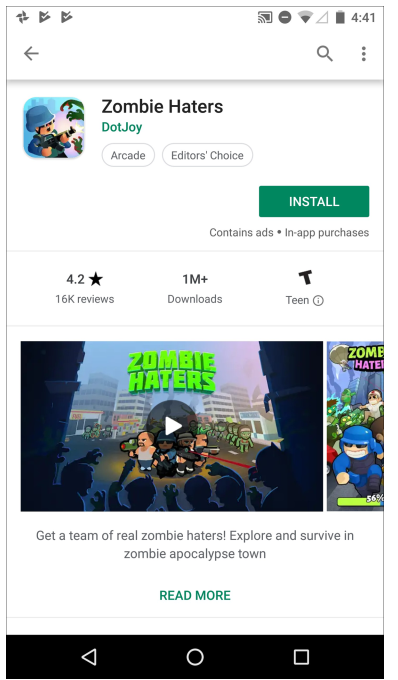
\includegraphics[scale=0.6]{images/lec08-pic09.png}
		\caption{Google Play store, Android OS mobile device}
	\end{figure}
\end{frame}

\begin{frame}[t]{Prominent <<Done>> Button or Assumed Next Step}
	\begin{itemize}
		\item выеделение цветом;
		\item кнопка, а не метка/ссылка;		
		\item кнопка окружена пустым пространством;		
		\item расположение кнопки указывает на переход на следующий шаг.		
	\end{itemize}
	
	\begin{figure}[h]
		\centering
		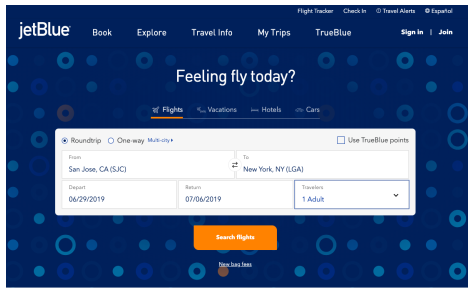
\includegraphics[scale=0.6]{images/lec08-pic10.png}
		\caption{JetBlue.com}
	\end{figure}
\end{frame}

\begin{frame}[t]{Prominent <<Done>> Button or Assumed Next Step}
	\begin{figure}[h]
		\centering
		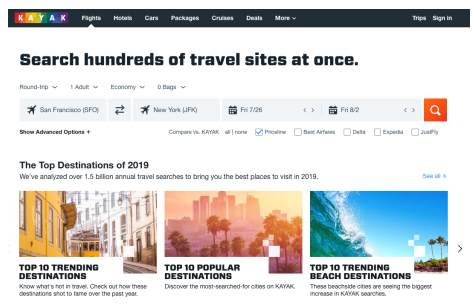
\includegraphics[scale=0.7]{images/lec08-pic11.png}
		\caption{Kayak.com}
	\end{figure}
\end{frame}

\begin{frame}[t]{Prominent <<Done>> Button or Assumed Next Step}
	\begin{figure}[h]
		\centering
		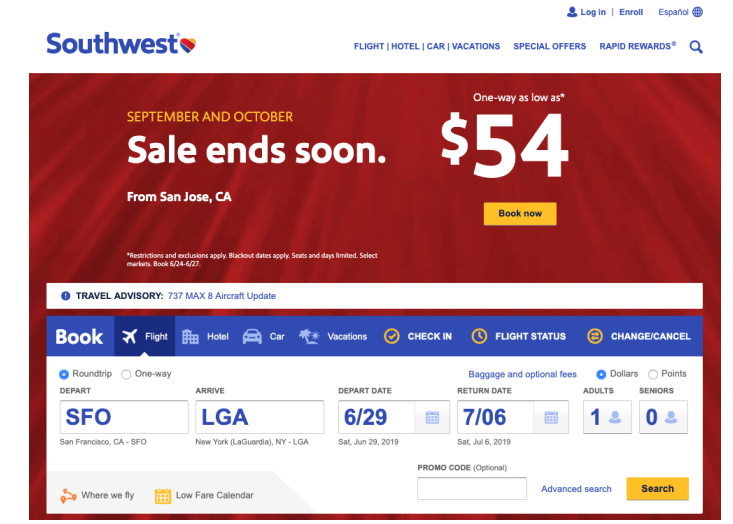
\includegraphics[scale=0.6]{images/lec08-pic12.png}
		\caption{Southwest.com}
	\end{figure}
\end{frame}

\begin{frame}[t]{Prominent <<Done>> Button or Assumed Next Step}
	\begin{figure}[h]
		\centering
		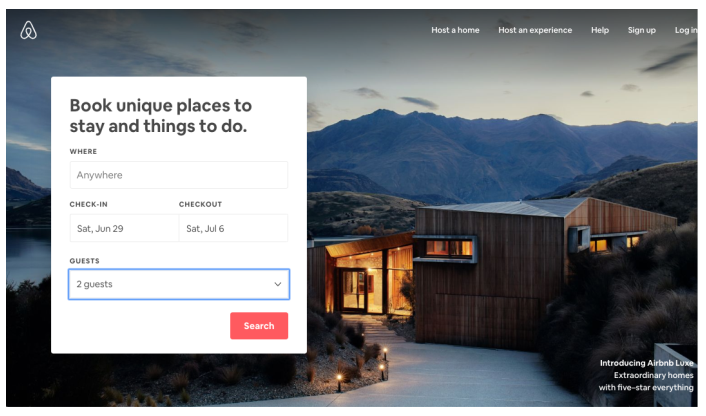
\includegraphics[scale=0.6]{images/lec08-pic13.png}
		\caption{Airbnb.com}
	\end{figure}
\end{frame}

\begin{frame}[t]{Smart Menu Items}
	В интерфейсе есть пункты меню, ведут себя немного по-разному в разных контекстах.
	
	\textbf{Шаблон}: Метки меню динамически изменяются (self-explain UI). 
	\begin{figure}[h]
		\centering
		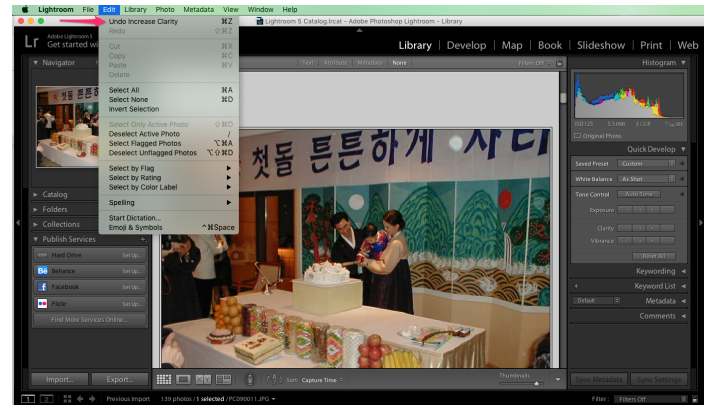
\includegraphics[scale=0.6]{images/lec08-pic14.png}
		\caption{Adobe Lightroom}
	\end{figure}
\end{frame}

\begin{frame}[t]{Smart Menu Items}
	\begin{itemize}
		\item Add [person from email] to Contacts list
		\item Add sender to Contacts list.
	\end{itemize}
	\begin{figure}[h]
		\centering
		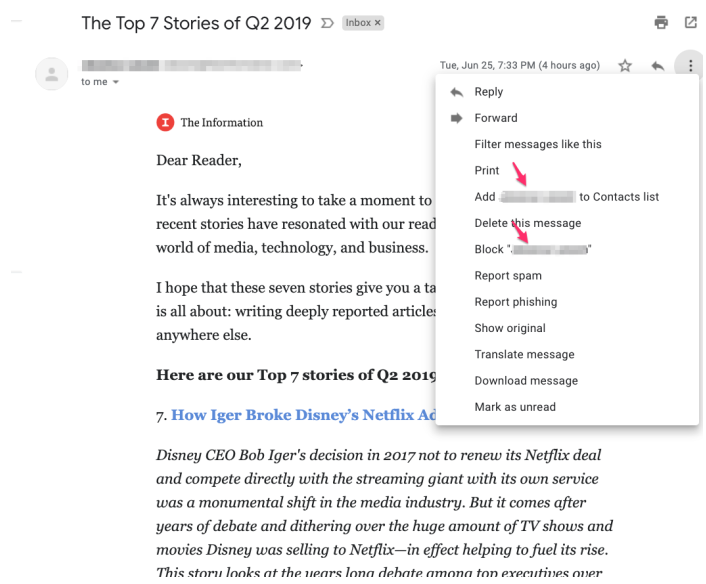
\includegraphics[scale=0.6]{images/lec08-pic15.png}
		\caption{GMail}
	\end{figure}
\end{frame}

\begin{frame}[t]{Preview}
	Пользователь собирается выполнить <<сложное>> действие -- открыть большой файл, распечатать 10-страничный документ, отправить форму анкету, совершить покупку.
	
	\textbf{Шаблон}: Визуализируйте облегченный образец команды или вероятных результатов действия.
	\begin{figure}[h]
		\centering
		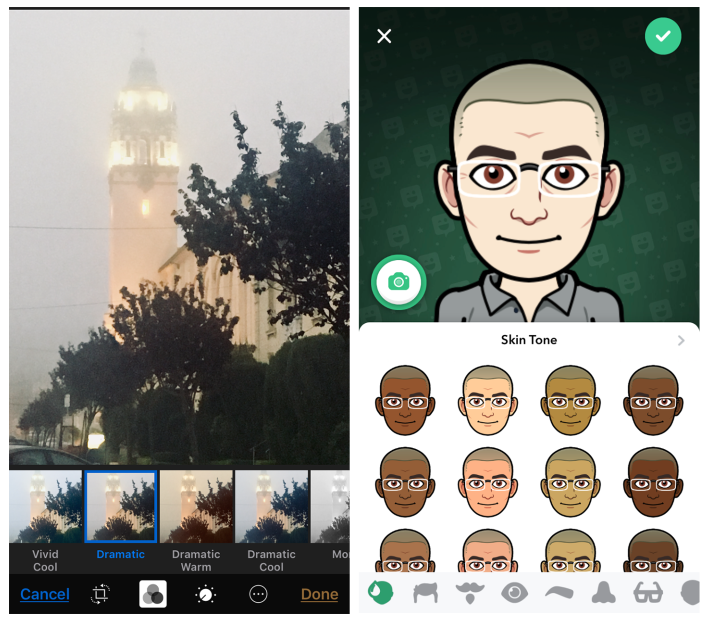
\includegraphics[scale=0.3]{images/lec08-pic16.png}
		\caption{Apple Photos app and Bitmoji app}
	\end{figure}
\end{frame}

\begin{frame}[t]{Preview}
	\begin{figure}[h]
		\centering
		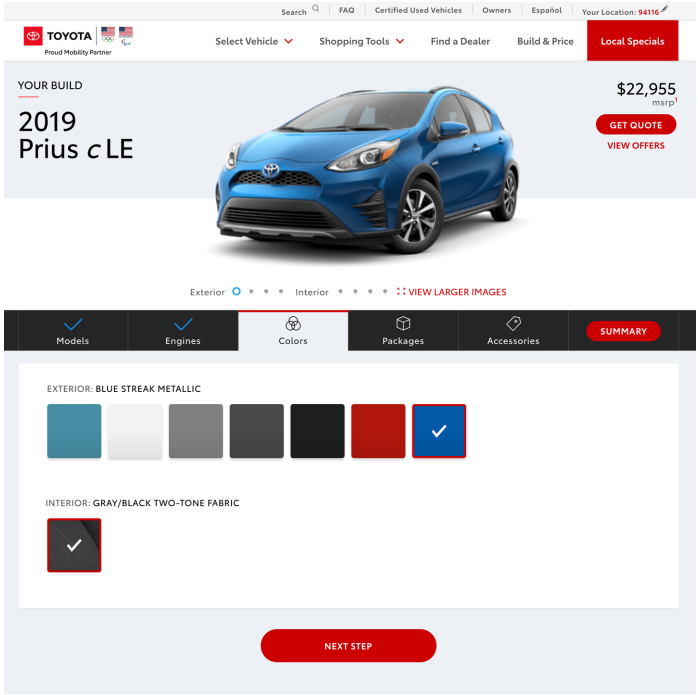
\includegraphics[scale=0.35]{images/lec08-pic17.png}
		\caption{Toyota.com}
	\end{figure}
\end{frame}

\begin{frame}[t]{Preview}
	\begin{figure}[h]
		\centering
		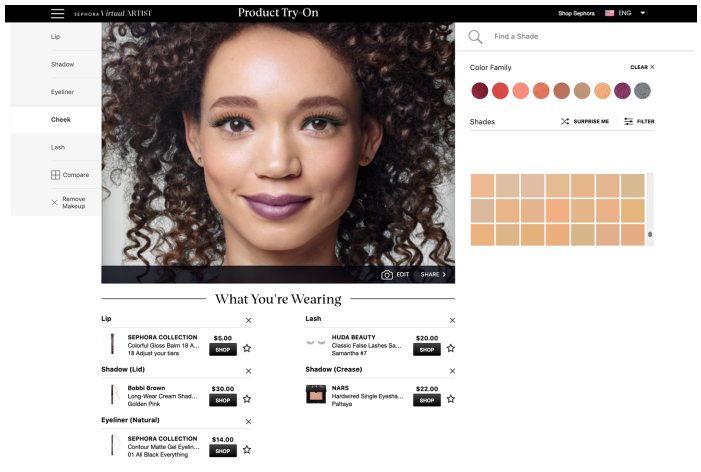
\includegraphics[scale=0.5]{images/lec08-pic18.png}
		\caption{Sephora.com}
	\end{figure}
\end{frame}

\begin{frame}[t]{Spinners and Loading Indicators}
	Длительная операция не позволяет взаимодействие с UI или выполняется в фоновом режиме более чем на две секунды.
	
	\textbf{Шаблон}: Анимация или другой индикатор, который отображается после отправки пользователем действия и до получения ответа.
	\begin{figure}[h]
		\centering
		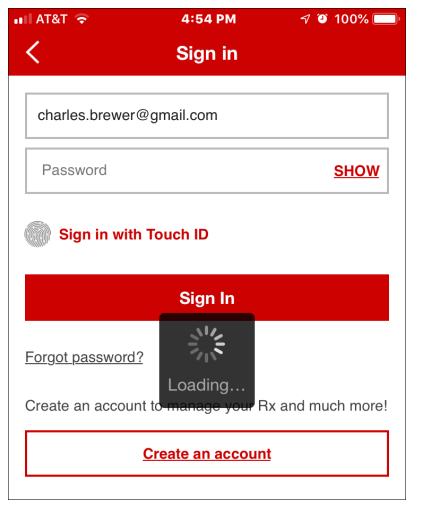
\includegraphics[scale=0.4]{images/lec08-pic19.png}
		\caption{Apple iOS, CVS mobile app; An iOS spinner example}
	\end{figure}
\end{frame}

\begin{frame}[t]{Spinners and Loading Indicators}
	\begin{figure}[h]
		\centering
		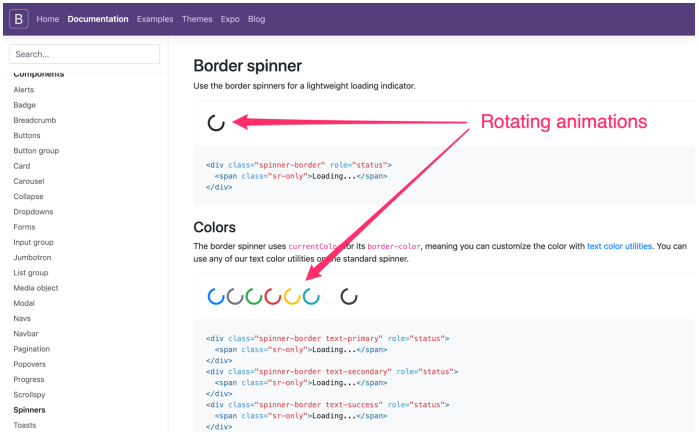
\includegraphics[scale=0.6]{images/lec08-pic20.png}
		\caption{Twitter Bootstrap component library (getbootstrap.com) border spinner}
	\end{figure}
\end{frame}

\begin{frame}[t]{Spinners and Loading Indicators}
	\begin{itemize}
		\item Что происходит в настоящее время?
		\item Какая часть операции завершена?
		\item Сколько времени осталось?
		\item Как это остановить?
	\end{itemize}

	\begin{figure}[h]
		\centering
		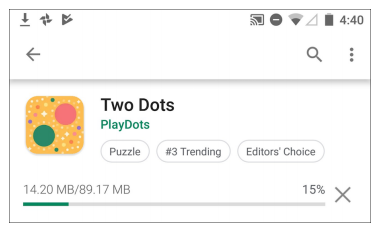
\includegraphics[scale=0.5]{images/lec08-pic21.png}
		\caption{Adobe Creative Cloud desktop manager, macOS}
	\end{figure}
\end{frame}

\begin{frame}[t]{Cancelability}
	Возможность мгновенно отменить трудоемкую операцию без каких-либо побочных эффектов.
	
	\begin{figure}[h]
		\centering
		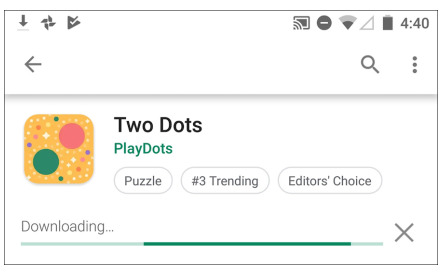
\includegraphics[scale=0.6]{images/lec08-pic22.png}
		\caption{Google Play store, Android OS}
	\end{figure}
\end{frame}

\begin{frame}[t]{Cancelability}
	\begin{figure}[h]
		\centering
		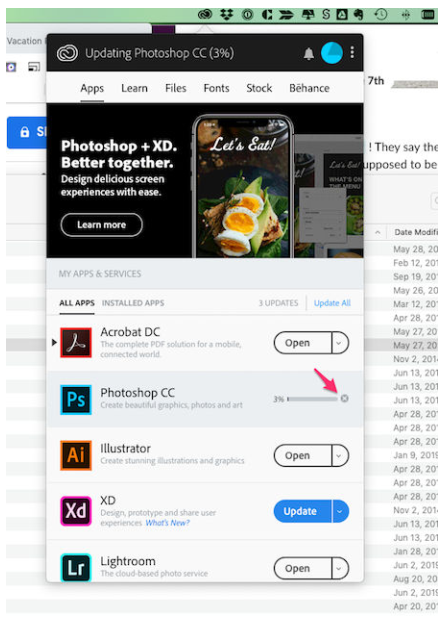
\includegraphics[scale=0.5]{images/lec08-pic23.png}
		\caption{Adobe Creative Cloud desktop manager, macOS}
	\end{figure}
\end{frame}

\begin{frame}[t]{Multilevel Undo}
	Вы создаете высокоинтерактивный пользовательский интерфейс, который является более сложным, чем простая навигация или заполнение форм.
	
	\textbf{Шаблон}: Возможность отменить ряд действий, выполняемых пользователем.
	\begin{figure}[h]
		\centering
		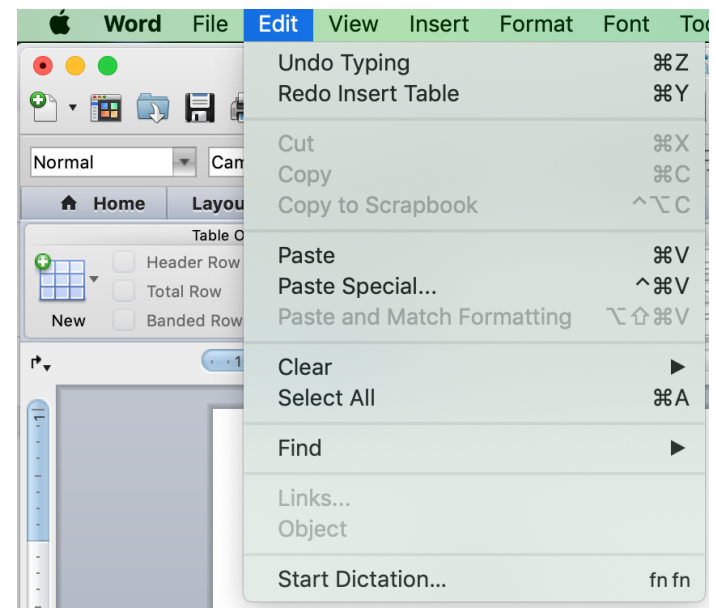
\includegraphics[scale=0.6]{images/lec08-pic24.png}
		\caption{Microsof Word History of Actions}
	\end{figure}
\end{frame}

\begin{frame}[t]{Multilevel Undo}
	Пользователь ожидает, что следующие действия он может отменить:
	\begin{itemize}
		\item Ввод текста для документов или электронных таблиц
		\item Модификации изображений или живописных полотен
		\item Изменения макета - положение, размер, порядок, группировка
		\item Файловые операции (удаление или переименование)
		\item Создание, удаление или перестановка объектов
		\item Любая операция вырезания, копирования или вставки
	\end{itemize}
	Следующие действия не отменяются:
	\begin{itemize}
		\item Выбор текста или объекта
		\item Навигация между окнами или страницами
		\item Расположение курсора мыши и текстового курсора
		\item Положение полосы прокрутки
		\item Положение и размеры окон или панелей
	\end{itemize}	
\end{frame}

\begin{frame}[t]{Command History}
	Пользователи выполняют длинные и сложные последовательности действий либо с помощью графического интерфейса, либо с помощью командной строки.
	
	\textbf{Шаблон}: Когда пользователь выполняет действия, ведите видимую запись этих действий - что и когда было сделано.
	\begin{figure}[h]
		\centering
		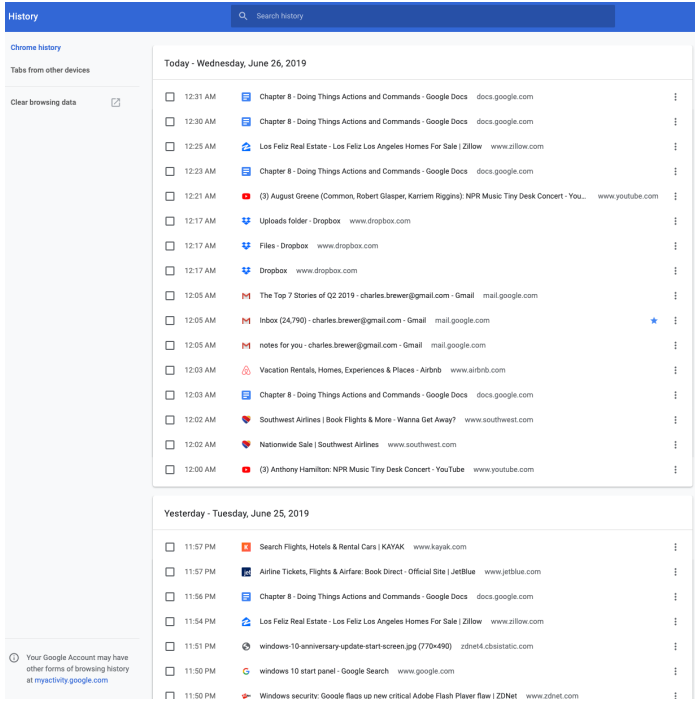
\includegraphics[scale=0.6]{images/lec08-pic25.png}
		\caption{Google Chrome History screen}
	\end{figure}
\end{frame}

\begin{frame}[t]{Command History}
	Для чего хранить историю команд?
	\begin{itemize}
		\item Повторить действие или команду, выполненные ранее
		\item Вспомнить порядок, в котором были сделаны некоторые действия
		\item Повторить последовательность операций, первоначально выполненных с одним объектом, на другом объекте
		\item Вести журнал своих действий 
		\item Преобразование интерактивной серии команд в сценарий или макрос
	\end{itemize}
\end{frame}

\begin{frame}[t]{Command History}
	\begin{figure}[h]
		\centering
		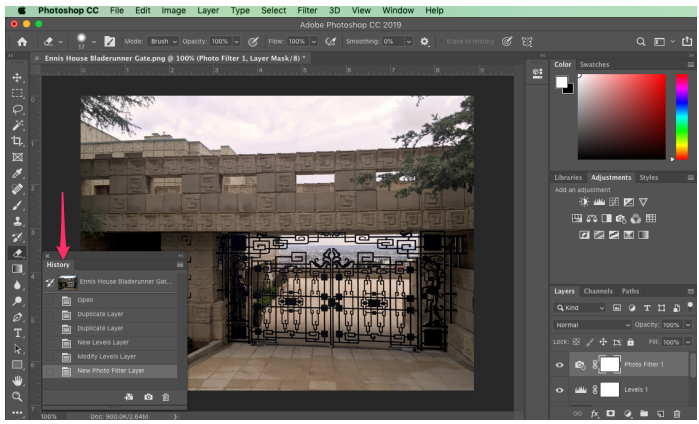
\includegraphics[scale=0.5]{images/lec08-pic26.png}
		\caption{Adobe Photoshop CC}
	\end{figure}
\end{frame}

\begin{frame}[t]{Macros}
	Пользователи могут захотеть повторить длинные последовательности действий или команд.
	
	\textbf{Шаблон}: Макросы -- это отдельные действия, состоящие из других, меньших действий. Пользователи могут создавать их путем записи или объединения последовательностей действий.
	\begin{figure}[h]
		\centering
		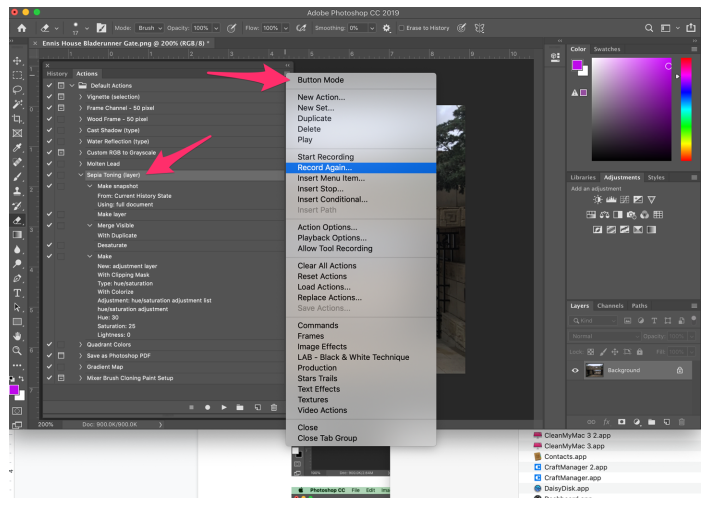
\includegraphics[scale=0.35]{images/lec08-pic27.png}
		\caption{Recording a macro in Adobe Photoshop CC}
	\end{figure}
\end{frame}

\begin{frame}[t]{Macros}
	\begin{figure}[h]
		\centering
		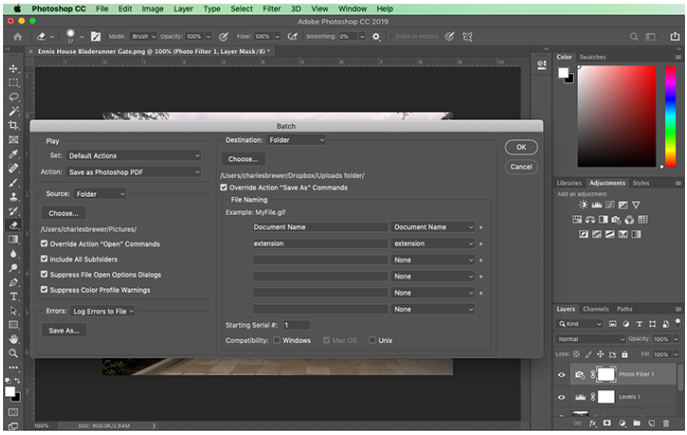
\includegraphics[scale=0.5]{images/lec08-pic28.png}
		\caption{Batch automation: confguring a series of actions to perform on multiple files automatically}
	\end{figure}
\end{frame}

\section{Формы и элементы управления}

%Respect the user’s time and attention
%Make sure the user understands the purpose of the form
%Minimize the number of form inputs
%Minimize visual clutter
%Group and title the form elements into sections where possible
%Consider dynamic, show/hide sections for long, complicated forms
%Use alignment for clear vertical flow
%Indicate what are required and what are optional felds
%Labels, instructions, examples, and help
%Use the width of the input felds to preview the length of the input
%Accept variations in input formatting
%Error prevention and validation as quickly as possible
%Consider top-aligned labels for mobile and web-responsive designs
%Consider internationalization
%Message success
%Usability test it

\begin{frame}[t]{Forgiving Format}
	Ваш пользовательский интерфейс запрашивает данные, которые пользователи могут вводить с непредсказуемым сочетанием словаря
или стиля (пробелы, дефисы, аббревиатуры или заглавные буквы).
	\begin{figure}[h]
		\centering
		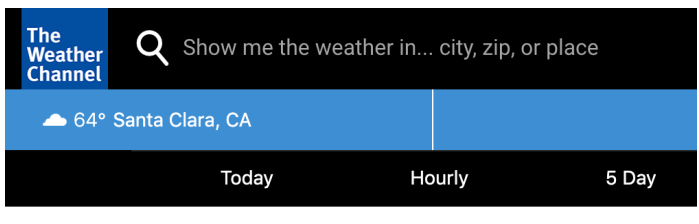
\includegraphics[scale=0.6]{images/lec08-pic30.png}
		\caption{Weather.com}
	\end{figure}
\end{frame}
	
\begin{frame}[t]{Forgiving Format}
	Разрешите пользователям вводить входные данные в различных вариантах, форматах и синтаксисе и заставьте
приложение обрабатывать их.
	
	\begin{figure}[h]
		\centering
		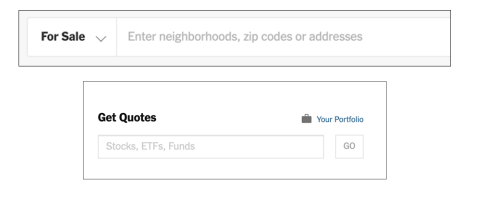
\includegraphics[scale=0.6]{images/lec08-pic31.png}
		\caption{Two search felds in the New York Times website hint at the variety of possible formats they will accept}
	\end{figure}	
\end{frame}

\begin{frame}[t]{Forgiving Format}
	\begin{figure}[h]
		\centering
		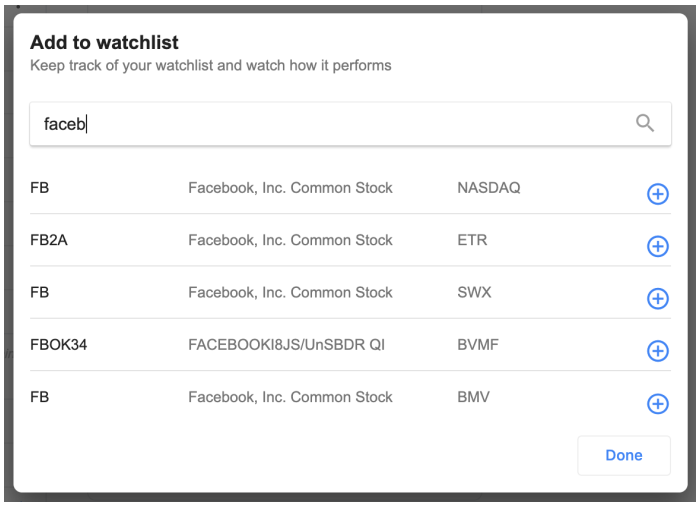
\includegraphics[scale=0.4]{images/lec08-pic32.png}
		\caption{Adding a stock to a personal watchlist in Google Finance}
	\end{figure}
\end{frame}

\begin{frame}[t]
	\begin{figure}[h]
		\centering
		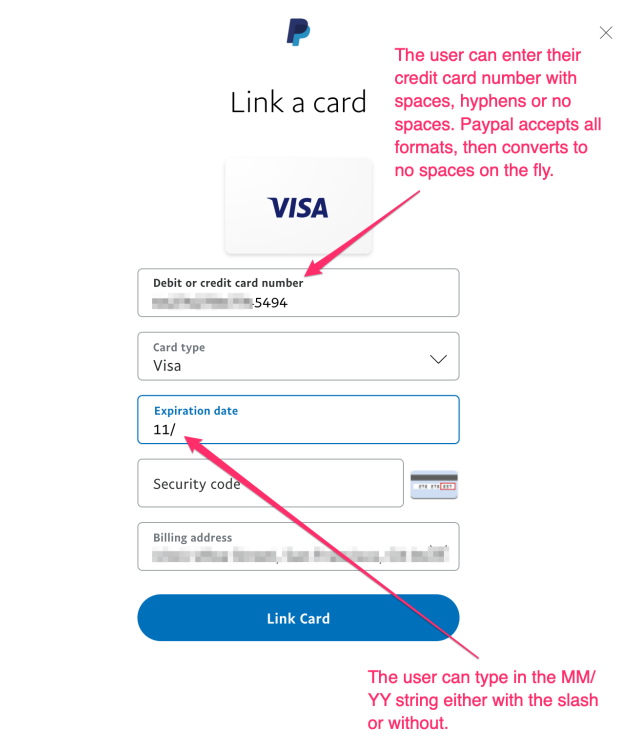
\includegraphics[scale=0.4]{images/lec08-pic33.png}
		\caption{PayPal}
	\end{figure}
\end{frame}

\begin{frame}[t]{Forgiving Format}
	\begin{figure}[h]
		\centering
		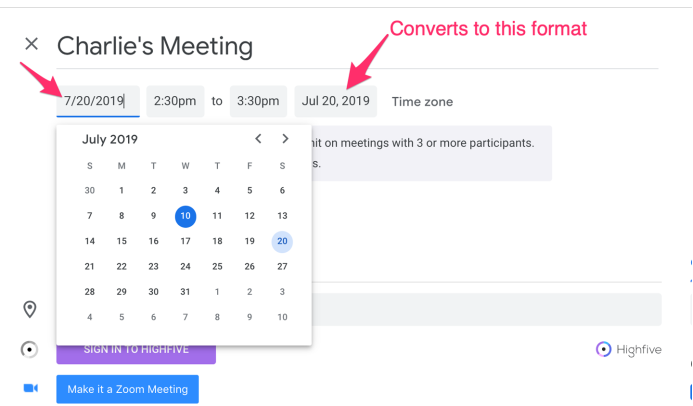
\includegraphics[scale=0.5]{images/lec08-pic34.png}
		\caption{Google Calendar}
	\end{figure}
\end{frame}

\begin{frame}[t]{Structured Format}
	\begin{figure}[h]
		\centering
		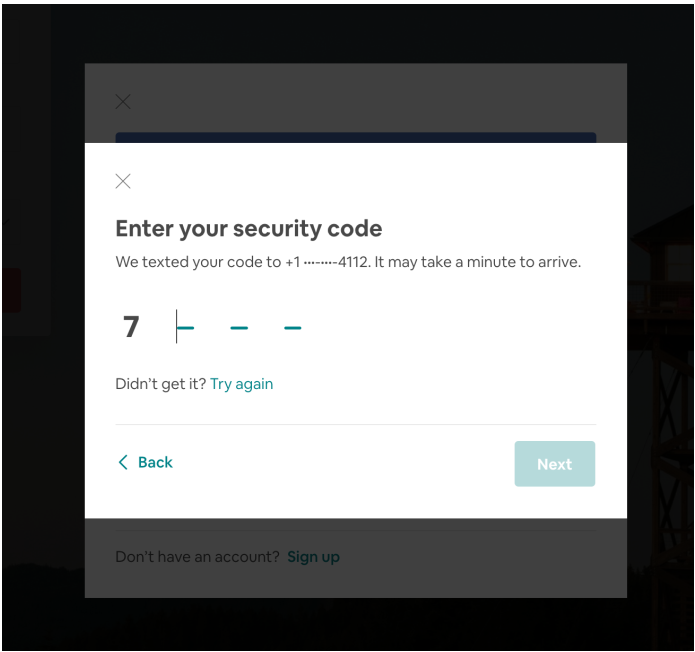
\includegraphics[scale=0.35]{images/lec08-pic35.png}
		\caption{Airbnb security code entry form}
	\end{figure}
\end{frame}

\begin{frame}[t]{Structured Format}
	Ваш интерфейс запрашивает у пользователя определенный текст, отформатированный определенным образом.
	
	\textbf{Шаблон:} Вместо одного текстового поля используйте набор текстовых полей, отражающих структуру запрашиваемых данных.
	\begin{figure}[h]
		\centering
		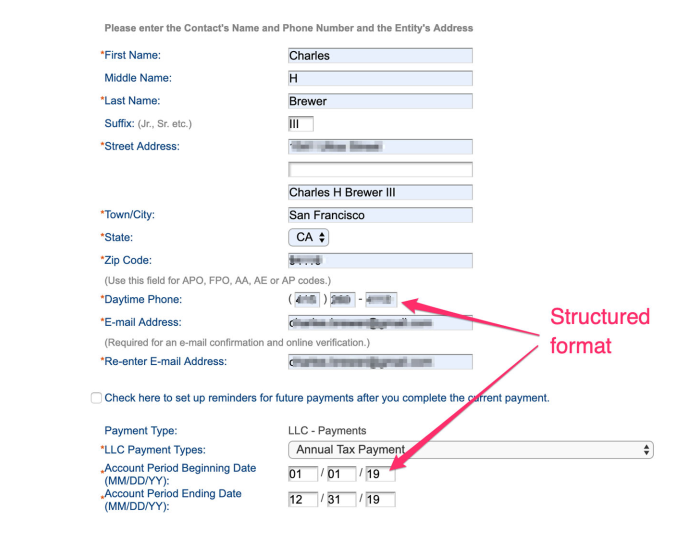
\includegraphics[scale=0.3]{images/lec08-pic36.png}
		\caption{Ocialpayments.com}
	\end{figure}
\end{frame}

\begin{frame}[t]{Structured Format}
	\begin{figure}[h]
		\centering
		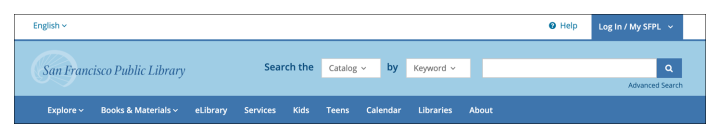
\includegraphics[scale=0.4]{images/lec08-pic37.png}
		\caption{San Francisco Public Library}
	\end{figure}

	\begin{figure}[h]
		\centering
		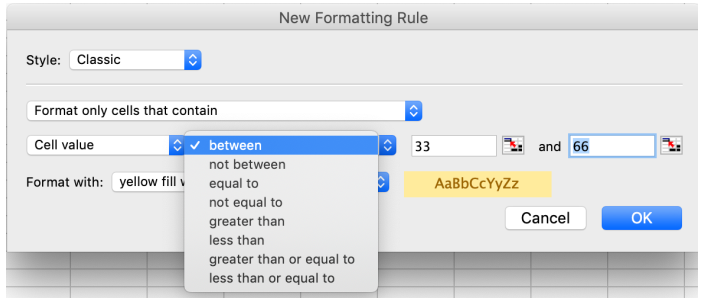
\includegraphics[scale=0.4]{images/lec08-pic38.png}
		\caption{Classic conditional fomatting in Microsof Excel}
	\end{figure}
\end{frame}

\begin{frame}[t]{Structured Format}
	\begin{figure}[h]
		\centering
		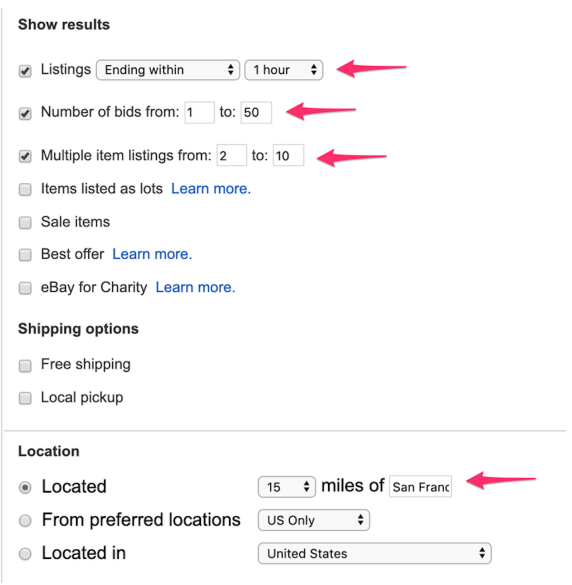
\includegraphics[scale=0.4]{images/lec08-pic40.png}
		\caption{eBay search flter form}
	\end{figure}
\end{frame}

\begin{frame}[t]{Input Hints}
	Интерфейс представляет собой текстовое поле, но тип ввода, который он требует, не очевиден для всех
пользователей.

	\textbf{Шаблон:} Рядом или под пустым текстовым полем поместите фразу или пример, который объясняет, что
требуется.
	\begin{figure}[h]
		\centering
		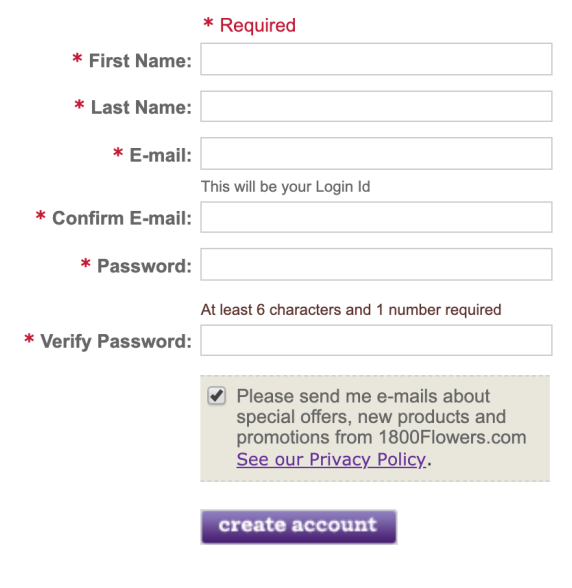
\includegraphics[scale=0.3]{images/lec08-pic41.png}
		\caption{The 1-800-Flowers registration screen}
	\end{figure}
\end{frame}

\begin{frame}[t]{Input Hints}	
	\begin{figure}[h]
		\centering
		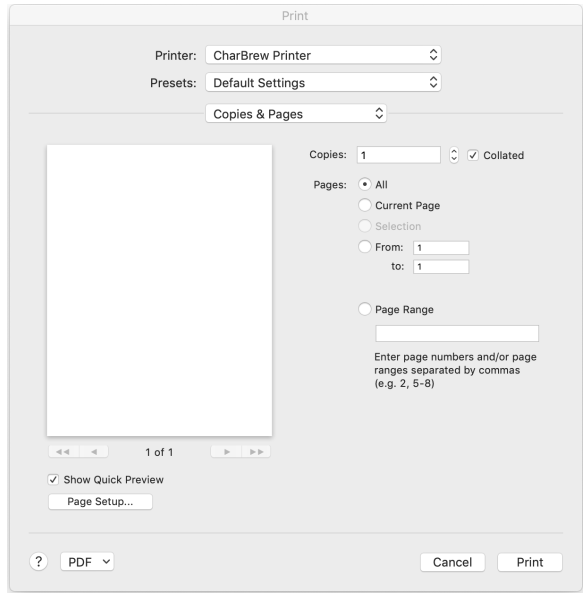
\includegraphics[scale=0.4]{images/lec08-pic42.png}
		\caption{Microsoft Word print dialog box}
	\end{figure}
\end{frame}

\begin{frame}[t]{Input Hints}
	\begin{figure}[h]
		\centering
		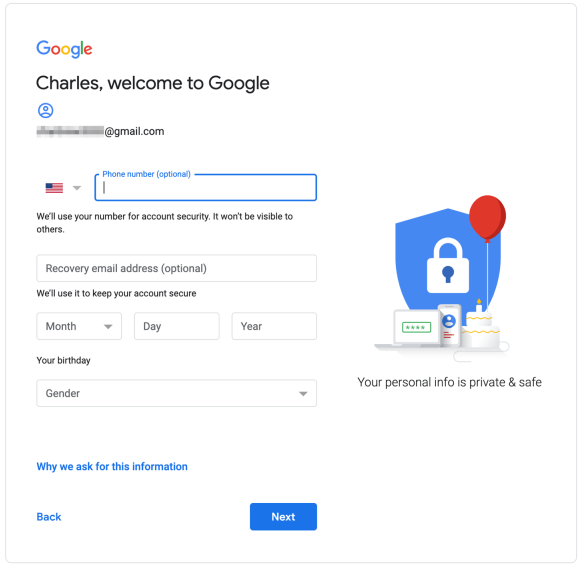
\includegraphics[scale=0.4]{images/lec08-pic43.png}
		\caption{Gmail registration page}
	\end{figure}
\end{frame}

\begin{frame}[t]{Input Hints}
	\begin{figure}[h]
		\centering
		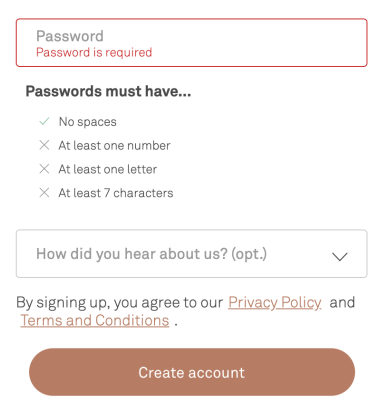
\includegraphics[scale=0.5]{images/lec08-pic45.png}
		\caption{Trunk Club}
	\end{figure}
\end{frame}

\begin{frame}[t]{Input Prompt}
	Пользовательский интерфейс представляет собой текстовое поле, раскрывающийся список или поле со списком для ввода.
	
	\textbf{Шаблон:} Предварительно заполните текстовое поле примером ввода или инструктивным текстом
	\begin{figure}[h]
		\centering
		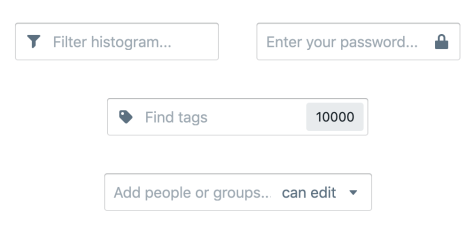
\includegraphics[scale=0.5]{images/lec08-pic46.png}
		\caption{Blueprints UI Toolkit; four example inputs with prompts}
	\end{figure}
\end{frame}

\begin{frame}[t]{Input Prompt}
	\begin{figure}[h]
		\centering
		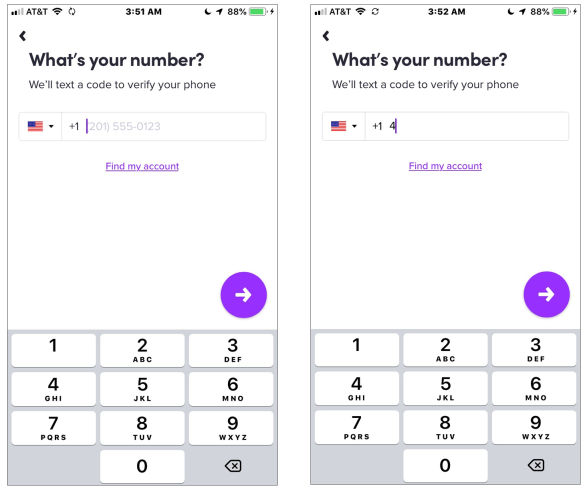
\includegraphics[scale=0.5]{images/lec08-pic47.png}
		\caption{Lyft mobile app input prompt}
	\end{figure}
\end{frame}

\begin{frame}[t]{Password Strength Meter}
	Пользовательский интерфейс просит пользователя выбрать новый пароль.
	
	\textbf{Шаблон:} Дайте пользователю немедленную обратную связь о новом пароле во время его ввода.
	\begin{figure}[h]
		\centering
		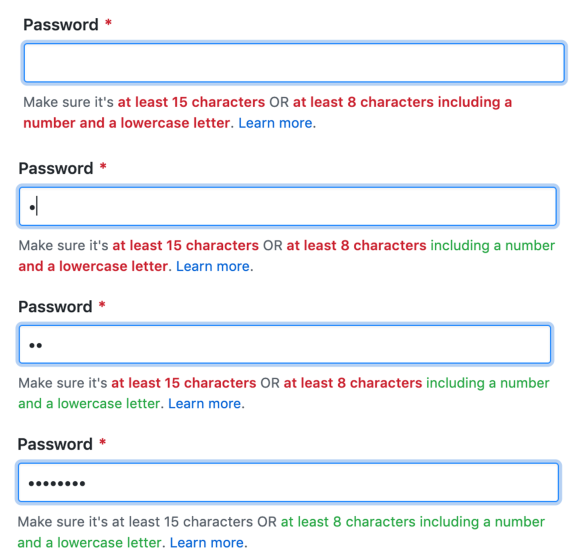
\includegraphics[scale=0.3]{images/lec08-pic48.png}
		\caption{GitHub password strength meter states}
	\end{figure}
\end{frame}

\begin{frame}[t]{Password Strength Meter}
	\begin{figure}[h]
		\centering
		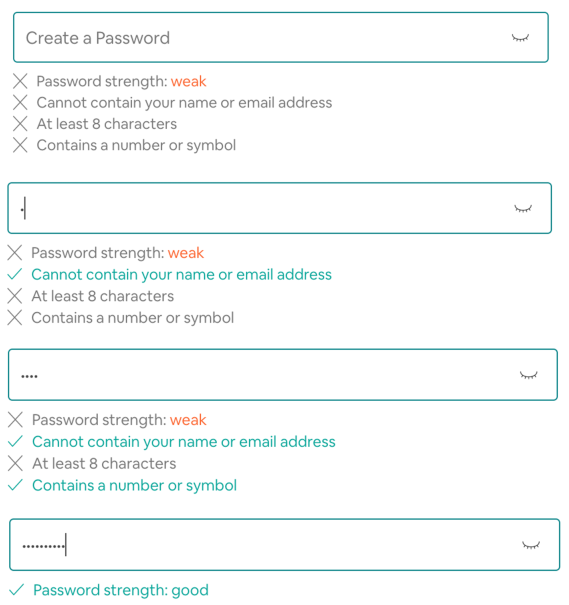
\includegraphics[scale=0.4]{images/lec08-pic49.png}
		\caption{Airbnb password strength meter states}
	\end{figure}
\end{frame}

\begin{frame}[t]{Autocompletion}
	Когда пользователь вводит текст в текстовое поле, предвосхищайте возможные ответы, показывайте них и автоматически завершайте ввод, когда это необходимо.
	\begin{figure}[h]
		\centering
		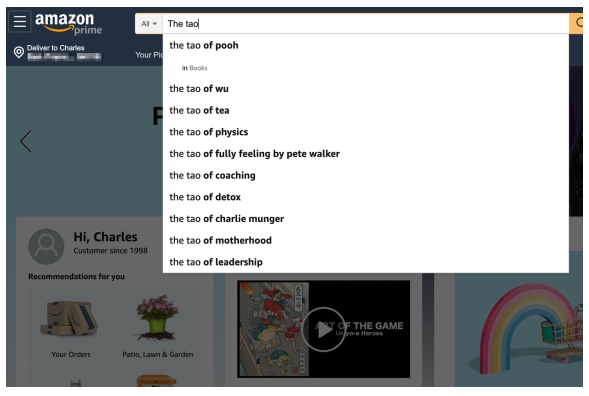
\includegraphics[scale=0.4]{images/lec08-pic50.png}
		\caption{Amazon autocomplete}
	\end{figure}
\end{frame}

\begin{frame}[t]
	\begin{figure}[h]
		\centering
		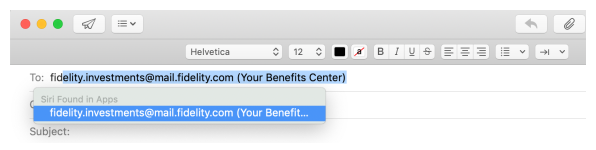
\includegraphics[scale=0.4]{images/lec08-pic51.png}
		\caption{Apple Mail autocomplete}
	\end{figure}

	\begin{figure}[h]
		\centering
		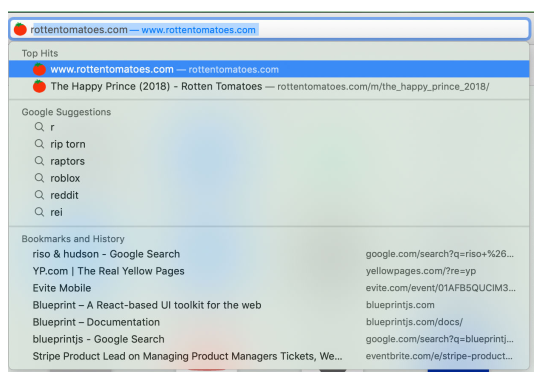
\includegraphics[scale=0.4]{images/lec08-pic52.png}
		\caption{Apple Safari browser autocomplete}
	\end{figure}
\end{frame}

\begin{frame}[t]{Autocompletion}
	\begin{figure}[h]
		\centering
		\includegraphics[scale=0.5]{images/lec08-pic53.png}
		\caption{Android Search autocomplete}
	\end{figure}
\end{frame}

\begin{frame}[t]{Autocompletion}
	\begin{figure}[h]
		\centering
		\includegraphics[scale=0.6]{images/lec08-pic54.png}
		\caption{Yelp.com Search autocomplete}
	\end{figure}
\end{frame}

\begin{frame}[t]{Autocompletion}
	\begin{figure}[h]
		\centering
		\includegraphics[scale=0.6]{images/lec08-pic55.png}
		\caption{ Kayak.com Search autocomplete}
	\end{figure}
\end{frame}

\begin{frame}[t]{Drop-down Chooser}
	Пользователь должен выбрать элемент из заданного набора.
	
	\textbf{Шаблон}: раскрывающейся список, который содержит более сложный пользовательский интерфейс для выбора.
	\begin{figure}[h]
		\centering
		\includegraphics[scale=0.5]{images/lec08-pic56.png}
		\caption{Microsoft Word drop-down choosers}
	\end{figure}
\end{frame}

\begin{frame}[t]{Drop-down Chooser}
	\begin{figure}[h]
		\centering
		\includegraphics[scale=0.35]{images/lec08-pic57.png}
		\caption{Photoshop and Sketch drop-down choosers}
	\end{figure}
\end{frame}

\begin{frame}[t]{List Builder}
	Вы просите пользователя создать список элементов, выбрав их из другого списка. 
	
	Список источников может быть слишком длинным, чтобы его можно было легко отобразить в виде набора флажков.
	\begin{figure}[h]
		\centering
		\includegraphics[scale=0.5]{images/lec08-pic58.png}
		\caption{Loudev.com multiselect.js}
	\end{figure}
\end{frame}

\begin{frame}[t]{List Builder}
	\begin{figure}[h]
		\centering
		\includegraphics[scale=0.6]{images/lec08-pic59.png}
		\caption{Adobe Lightroom}
	\end{figure}
\end{frame}

\begin{frame}[t]{Good Defaults and Smart Prells}
	Ваш пользовательский интерфейс задает пользователю вопросы, требующие ввода в форме (например, текстовые поля или переключатели), и вы хотите уменьшить объем работы, которую должны выполнять пользователи.
	\begin{figure}[h]
		\centering
		\includegraphics[scale=0.4]{images/lec08-pic60.png}
		\caption{1}
	\end{figure}
\end{frame}

\begin{frame}[t]{Good Defaults and Smart Prells}
	Используйте значения по умолчанию для элементов формы, которые cъэкономят временя и усилия пользователя при заполнении формы.
	\begin{figure}[h]
		\centering
		\includegraphics[scale=0.5]{images/lec08-pic61.png}
		\caption{A Create New dialog in Photoshop CC}
	\end{figure}
\end{frame}

\begin{frame}[t]{Good Defaults and Smart Prells}
	\begin{figure}[h]
		\centering
		\includegraphics[scale=0.4]{images/lec08-pic62.png}
		\caption{Canvas Size dialog box in Photoshop CC}
	\end{figure}
\end{frame}

\begin{frame}[t]{Error Messages}
	Пользователи могут вводить информацию о форме, которая каким-то образом неприемлема. Они могут:
	\begin{itemize}
		\item пропустить обязательные поля; 
		\item ввести некорректные данные;
		\item ввести недопустимые адреса электронной почты и т.д.
	\end{itemize}
	\begin{figure}[h]
		\centering
		\includegraphics[scale=0.3]{images/lec08-pic63.png}
		\caption{Mailchimp registration page}
	\end{figure}
\end{frame}

\begin{frame}[t]{Error Messages}
	Если есть ошибка ввода, поместите привлекающее внимание пояснительное сообщение об ошибке непосредственно на саму форму.
	\begin{figure}[h]
		\centering
		\includegraphics[scale=0.3]{images/lec08-pic64.png}
		\caption{Mint (Intuit) and H and M registration screen}
	\end{figure}
\end{frame}

\begin{frame}[t]{Error Messages}
	\begin{figure}[h]
		\centering
		\includegraphics[scale=0.5]{images/lec08-pic65.png}
		\caption{Twitter registration}
	\end{figure}
\end{frame}

\begin{frame}[t]{Error Messages}
	\begin{figure}[h]
		\centering
		\includegraphics[scale=0.4]{images/lec08-pic66.png}
		\caption{Jos. A. Bank}
	\end{figure}
\end{frame}

\end{document}
